\documentclass[11pt,a4paper]{article}
\usepackage[utf8]{inputenc}
\usepackage[vietnamese]{babel}
\usepackage{amsmath,amssymb}
\usepackage[version=4]{mhchem}
\usepackage{geometry}
\geometry{top=1.5cm,bottom=1.2cm,left=1.4cm,right=1.4cm,headheight=28pt,headsep=12pt,footskip=18pt}
\usepackage{graphicx}
\usepackage{xcolor}
\usepackage{tabularx}
\usepackage{array}
\usepackage{colortbl}
\usepackage{tikz}
\usepackage{chemfig}
\usepackage{fancyhdr}
\usepackage{enumitem}
\usepackage{multido}
\usepackage{tcolorbox}

\definecolor{hfRed}{HTML}{D32F2F}
\definecolor{hfGreen}{HTML}{8BC390}
\definecolor{mainGreen}{HTML}{2E7D32}
\definecolor{solBlue}{HTML}{1565C0}
\definecolor{tableGreen}{HTML}{E8F5E9}

\usepackage{ex_test}

\pagestyle{fancy}
\fancyhf{}
\renewcommand{\headrulewidth}{0.75pt}
\renewcommand{\headrule}{\hbox to\headwidth{\color{hfGreen}\leaders\hrule height \headrulewidth\hfill}}
\renewcommand{\footrulewidth}{0.75pt}
\renewcommand{\footrule}{\hbox to\headwidth{\color{hfGreen}\leaders\hrule height \footrulewidth\hfill}}

\fancyhead[L]{\small\itshape\color{hfRed}Tài liệu lưu hành nội bộ}
\fancyhead[R]{\small\color{hfRed}Thầy \textbf{TRẦN VĂN THẠNH} - 0777.470.803}

\fancyfoot[L]{\footnotesize\itshape\color{hfRed}CS1: 6/15 Nguyễn Hoàng, P. Kim Long, TP Huế \quad|\quad CS2: 24 Đặng Thái Thân, TP Huế}
\fancyfoot[R]{\small\textbf{\color{hfRed}Trang \thepage}}

\setlength{\parindent}{0pt}
\setlength{\parskip}{2pt}

\begin{document}

\begin{minipage}[t]{0.48\textwidth}
\textbf{SỞ GD \& ĐT THÀNH PHỐ HUẾ}\\
\textbf{TRƯỜNG THPT GIA HỘI}\\
\textit{ĐỀ CHÍNH THỨC}\\
\textit{(Đề thi có 03 trang)}
\end{minipage}
\hfill
\begin{minipage}[t]{0.48\textwidth}
\raggedleft
\textbf{\color{hfRed}KIỂM TRA GIỮA KÌ II}\\
\textbf{NĂM HỌC 2025 -- 2026}\\
\textbf{MÔN: HOÁ HỌC LỚP 11}\\
\textit{Thời gian làm bài: 45 phút (không kể thời gian phát đề)}\\
\textbf{MÃ ĐỀ THI: 2608}
\end{minipage}

\vspace{4pt}
\noindent
\textit{Họ tên thí sinh:} \dotfill \textit{Lớp:} \dotfill \textit{Số báo danh:} \dotfill

\vspace{3pt}
\noindent
\textit{\footnotesize Cho nguyên tử khối của các nguyên tố: $\ce{H}=1; \ce{C}=12; \ce{O}=16; \ce{Cl}=35{,}5; \ce{Ag}=108; \ce{Br}=80; \ce{N}=14$.}

\vspace{3pt}
\hrule color{hfGreen} height 0.5pt

\vspace{4pt}
\noindent
{\color{mainGreen}\textbf{\large I. TRẮC NGHIỆM NHIỀU LỰA CHỌN: (12 câu -- 3,0 điểm)}}\\
\textit{\small (Học sinh chọn đáp án đúng nhất. Mỗi câu trả lời đúng được 0,25 điểm)}
\vspace{2pt}

\begin{ex}
Phản ứng thế giữa 2,3-dimethylbutane với $\ce{Cl2}$ (tỉ lệ mol 1:1) cho mấy sản phẩm thế?
\choice
{\True 2.}
{5.}
{3.}
{4.}
\end{ex}
\begin{ex}
Cho 5 chất: $\ce{CH3CH2CH2Cl}$ (1); $\ce{CH2=CHCH2Cl}$ (2); $\ce{C6H5Cl}$ (3); $\ce{CH2=CHCl}$ (4); $\ce{C6H5CH2Cl}$ (5). Đun từng chất với dung dịch $\ce{NaOH}$ loãng, dư, sau đó gạn lấy lớp nước và acid hoá bằng dung dịch $\ce{HNO3}$, sau đó nhỏ vào đó dung dịch $\ce{AgNO3}$ thì các chất có xuất hiện kết tủa trắng là
\choice
{(1), (2), (3), (5).}
{\True (1), (2), (5).}
{(2), (3), (5).}
{(1), (3), (5).}
\end{ex}
\begin{ex}
Cho dãy các chất: (a) toluene; (b) \textit{o}-xylene; (c) ethylbenzene; (d) \textit{m}-dimethylbenzene; (e) styrene. Những chất đồng đẳng của benzene là
\choice
{(a), (b), (c), (e).}
{(a), (d).}
{\True (a), (b), (c), (d).}
{(a), (e).}
\end{ex}
\begin{ex}
Ethyl chloride được dùng làm thuốc xịt có tác dụng giảm đau tạm thời khi chơi thể thao. Công thức phân tử của ethyl chloride là
\choice
{$\ce{C2H5F}$.}
{$\ce{C2H3Cl}$.}
{$\ce{CH3Cl}$.}
{\True $\ce{C2H5Cl}$.}
\end{ex}
\begin{ex}
Dẫn xuất halogen của hydrocarbon không chứa nguyên tố nào sau đây?
\choice
{Chlorine.}
{Bromine.}
{\True Oxygen.}
{Fluorine.}
\end{ex}
\begin{ex}
Cho $\ce{X}$ có công thức cấu tạo: $\ce{CH3-CH=C(CH3)-CH3}$. Danh pháp thay thế của $\ce{X}$ là
\choice
{3-methylbut-3-ene.}
{\True 2-methylbut-2-ene.}
{3-methylbut-2-ene.}
{2-methylbut-3-ene.}
\end{ex}
\begin{ex}
Đặc điểm nào sau đây là của hydrocarbon no?
\choice
{Chỉ có liên kết đôi.}
{Có ít nhất một vòng no.}
{Có ít nhất một liên kết đôi.}
{\True Chỉ có liên kết đơn.}
\end{ex}
\begin{ex}
Cho các dẫn xuất halogen của hydrocarbon sau: $\ce{C2H5F}$ (1); $\ce{C2H5Br}$ (2); $\ce{C2H5I}$ (3); $\ce{C2H5Cl}$ (4). Thứ tự giảm dần nhiệt độ sôi là
\choice
{(1) $>$ (4) $>$ (2) $>$ (3).}
{\True (3) $>$ (2) $>$ (4) $>$ (1).}
{(1) $>$ (2) $>$ (3) $>$ (4).}
{(3) $>$ (2) $>$ (1) $>$ (4).}
\end{ex}
\begin{ex}
Alkyne là các hydrocarbon không no, mạch hở, có công thức chung là
\choice
{\True $\ce{C_n H_{2n-2}}$ ($n \ge 2$).}
{$\ce{C_n H_{2n}}$ ($n \ge 2$).}
{$\ce{C_n H_{2n+2}}$ ($n \ge 1$).}
{$\ce{C_n H_{2n}}$ ($n \ge 3$).}
\end{ex}
\begin{ex}
Benzene tác dụng được với chất nào sau đây ở điều kiện thích hợp?
\choice
{Dung dịch $\ce{Br2}$.}
{Dung dịch $\ce{NaOH}$.}
{\True $\ce{Br2}/\ce{FeBr3}, t^\circ$.}
{$\ce{NaCl}$ khan.}
\end{ex}
\begin{ex}
Cho sơ đồ phản ứng sau: $\ce{CH3-C#CH + AgNO3/NH3 -> X + NH4NO3}$. $\ce{X}$ có công thức cấu tạo là
\choice
{\True $\ce{CH3-C#C-Ag}$.}
{$\ce{CH3-C-Ag#C-Ag}$.}
{$\ce{CAg#CAg}$.}
{$\ce{Ag-CH2-C#C-Ag}$.}
\end{ex}
\begin{ex}
Ở điều kiện thường alkane nào sau đây ở thể lỏng?
\choice
{$\ce{C4H10}$.}
{$\ce{C3H8}$.}
{$\ce{C2H6}$.}
{\True $\ce{C6H14}$.}
\end{ex}
\vspace{4pt}
\noindent
{\color{mainGreen}\textbf{\large II. TRẮC NGHIỆM ĐÚNG-SAI: (2 câu -- 2,0 điểm)}}\\
\textit{\small (Trong mỗi ý (a), (b), (c), (d) ở mỗi câu, học sinh chọn đúng hoặc sai: Đ - S)}
\vspace{2pt}

\begin{ex}
Tiến hành thí nghiệm điều chế và thử tính chất của ethylene, người ta tiến hành các bước sau đây:
\begin{itemize}[leftmargin=1.2cm,itemsep=1pt]
\item \textbf{Bước 1:} Cho vào bình cầu khoảng 10 mL cồn $90^\circ$, thêm tiếp 5 mL dung dịch $\ce{H2SO4}$ đậm đặc và một ít đá bọt, lắc đều.
\item \textbf{Bước 2:} Chuẩn bị 2 bình thủy tinh, cho vào khoảng 5 mL dung dịch $\ce{NaOH}$ đặc vào bình (1) và khoảng 2 mL nước bromine vào bình (2).
\item \textbf{Bước 3:} Dùng đèn cồn đun nóng đều bình cầu; dẫn khí thu được lần lượt vào bình (1) sau đó vào bình (2).
\end{itemize}
\begin{center}
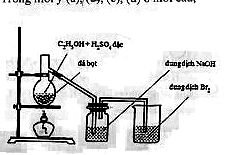
\includegraphics[width=0.48\textwidth]{images_gk2_hoa11_giahoi_2608/thi_nghiem_dieu_che_ethylene.png}
\end{center}
\choiceTF
{\True Vai trò của đá bọt là làm chất lỏng sôi đều và không bị trào ra.}
{Có thể thay dung dịch $\ce{H2SO4}$ đặc bằng dung dịch $\ce{H2SO4}$ 10\% vẫn thu được ethylene.}
{\True Khi ethylene sinh ra sẽ làm nhạt màu ống nghiệm đựng dung dịch $\ce{Br2}$, phản ứng xảy ra là phản ứng oxi hóa khử.}
{\True Trong phòng thí nghiệm, để thu khí ethylene, người ta dùng phương pháp đẩy nước.}
\end{ex}
\begin{ex}
Benzene, toluene và styrene đều thuộc hợp chất hydrocarbon thơm (Arene).
\choiceTF
{Benzene, toluene và styrene đều có công thức chung là $\ce{C_n H_{2n-6}}$ ($n \ge 6$).}
{Styrene còn có tên gọi khác là ethylbenzene.}
{\True Để phân biệt benzene, toluene và styrene có thể dùng dung dịch $\ce{KMnO4}$.}
{So với benzene thì toluene phản ứng thế nguyên tử hydrogen ở vòng benzene dễ dàng hơn so với benzene và sản phẩm chính ưu tiên thế vào vị trí meta (\textit{-m}).}
\end{ex}
\vspace{4pt}
\noindent
{\color{mainGreen}\textbf{\large III. TRẮC NGHIỆM TRẢ LỜI NGẮN: (4 câu -- 2,0 điểm)}}\\
\textit{\small (Thí sinh ghi đáp án ngắn gọn vào ô/dòng trả lời)}
\vspace{2pt}

\begin{ex}
Trong số các hydrocarbon mạch hở sau: $\ce{C2H2, C4H10, C4H6, C4H8, C3H4, C3H6}$. Có bao nhiêu hydrocarbon có thể tạo kết tủa với dung dịch $\ce{AgNO3/NH3}$?

\noindent\textit{Trả lời:} \dotfill
\end{ex}
\begin{ex}
Phần trăm khối lượng của carbon (\%C) có trong phân tử ethylbenzene là bao nhiêu? \textit{(làm tròn đến hàng phần mười)}.

\noindent\textit{Trả lời:} \dotfill
\end{ex}
\begin{ex}
Trong các chất: $\ce{CH3Cl; CH3NH2; CH4O; CH2Br2; C2H4Cl2, HCl, C6H5F}$ có bao nhiêu chất thuộc loại dẫn xuất halogen của hydrocarbon?

\noindent\textit{Trả lời:} \dotfill
\end{ex}
\begin{ex}
Da nhân tạo (PVC) được điều chế từ khí thiên nhiên theo sơ đồ:
$$\ce{CH4 -> C2H2 -> CH2=CH-Cl -> (-CH2-CHCl-)_n}$$
Nếu hiệu suất của toàn bộ quá trình điều chế là 20\%, muốn điều chế được 1,0 tấn PVC thì thể tích ($\text{m}^3$) khí thiên nhiên (chứa 80\% methane) ở điều kiện chuẩn cần dùng là bao nhiêu? \textit{(làm tròn kết quả đến hàng đơn vị)}.

\noindent\textit{Trả lời:} \dotfill
\end{ex}
\vspace{6pt}
\noindent
{\color{mainGreen}\textbf{\large IV. BÀI TẬP TỰ LUẬN: (3 câu -- 3,0 điểm)}}\\
\textit{\small (Học sinh trình bày chi tiết lời giải vào bài làm)}
\vspace{2pt}

\noindent
\textbf{Câu 1: (1,0 điểm)} Khí hóa lỏng hay khí gas (LPG -- Liquefied Petroleum Gas) được sử dụng làm nhiên liệu trong các hộ gia đình là propane hóa lỏng. Một bình khí gas hóa lỏng chứa 12,0 kg propane có thể cung cấp bao nhiêu Lít khí propane ở điều kiện chuẩn ($25^\circ\text{C}, 1\text{ bar}$)?

\vspace{2pt}
\noindent
\multido{\n=1+1}{6}{\dotfill\\[4pt]}

\vspace{4pt}
\noindent
\textbf{Câu 2: (1,0 điểm)} Nhựa PE (Polyethylene) là loại nhựa nhiệt dẻo phổ biến nhất thế giới, nổi bật với đặc tính dẻo dai, chống thấm nước, cách điện tốt và độ bền cao. Một trong những cách điều chế PE là theo sơ đồ: $\ce{C2H2 -> C2H4 -> polyethylene (PE)}$.\\
Viết các phương trình phản ứng thực hiện sơ đồ trên (ghi rõ điều kiện phản ứng).

\vspace{2pt}
\noindent
\multido{\n=1+1}{6}{\dotfill\\[4pt]}

\vspace{4pt}
\noindent
\textbf{Câu 3: (1,0 điểm)} Thuốc nổ TNT (2,4,6-trinitrotoluene) được điều chế bằng phản ứng của toluene với hỗn hợp gồm $\ce{HNO3}$ đặc và $\ce{H2SO4}$ đặc, trong điều kiện đun nóng. Biết hiệu suất của toàn bộ quá trình tổng hợp là 60\%. Lượng TNT (2,4,6-trinitrotoluene) tạo thành từ 552,0 gam toluene là bao nhiêu gam?

\vspace{2pt}
\noindent
\multido{\n=1+1}{6}{\dotfill\\[4pt]}

\vspace{8pt}
\begin{center}
\textbf{--------- HẾT ---------}
\end{center}

\end{document}
